\newpage\setcounter{section}{2}
\section{Tangent Vectors}

One of the very central ideas that we have in ordinary calculus is the idea of \textit{linear approximation}. In ordinary calculus, we approximated things by funding the tangent line to some curve at a specified point. However, to make sense of this notion for smooth manifolds, we need to talk about the idea of a \textit{tangent space to a manifold at a point}. The basic principles of these objects were introduced to us back in Calculus III when we learned about tangent vectors to curves and tangent planes to surfaces, so we will use this as the starting position for our discussion of geometric tangent vectors in $\Rn$.


\dfn Given a point $a\in \Rn$, let us define the \df{geometric tangent space to $\boldsymbol{\Rn}$ at a}, denoted by $\Rn_a$, to be the set $\{a\}\x \Rn$. A \df{geometric tangent vector} in $\Rn$ is an element of $\Rn_a$ for some $a\in \Rn$.

\dfn Given any geometric tangent vector $v_a\in \Rn_a$, we can define a map $D_v|_a:\Cin(\Rn)\ra \R$, which takes the directional derivative in the direction $v$ at $a$:
\[D_v|_a f = D_vf(a) = \ev{\frac{d}{dt}}{t = 0}f(a + tv).\]
If $v_a = v^ie_i|_a$ in terms of the standard basis, then by the chain rule, we can write
\[D_v|_af = v^i\pd{f}{x^i}(a).\]

\dfn A map $w:\Cin(\Rn)\ra \R$ is called a \df{derivation at a} if it is linear over $\R$ and satisfies the Leibniz rule:
\[w(fg) = f(a)wg + g(a)wf.\]
We will denote the set of all derivations of $\Cin(\Rn)$ at $a$ by $T_a\Rn$.

\begin{lem}[Properties of Derivations]
Suppose $a\in \Rn$, $w\in T_a\Rn$, and $f,g\in \Cin(\Rn)$.
\begin{enumerate}
    \item If $f$ is a constant function, then $wf = 0$.
    \item If $f(a) = g(a) = 0$ then $w(fg) = 0$.
\end{enumerate}
\end{lem}

\begin{prop}
Let $a\in \Rn$
\begin{enumerate}
    \item For each geometric tangent vector $v_a\in \Rn_a$, the map $D_v|_a:\Cin(\Rn)\ra \R$ is a derivation at $a$.
    \item The map $v_a\mapsto D_v|_a$ is an isomorphism form $\Rn_a$ onto $T_a\Rn$.
\end{enumerate}
\end{prop}

\begin{cor}
For any $a\in \Rn$, the $n$ derivations
\[\ev{\pdd{x^1}}{a},\ldots, \ev{\pdd{x^n}}{a}\quad\text{defined by}\quad \ev{\pdd{x^i}}{a}f = \pd{f}{x^i}(a)\]
form a basis for $T_a\Rn$, which therefore has dimension $n$.
\end{cor}

With this machinery out of the way, we are ready to generalize our notion of a tangent space to an arbitrary manifold.

\newpage

\subsection{Tangent Vectors on Manifolds}\nl

\dfn Let $M$ be a smooth manifold with or without boundary, and let $p$ be a point of $M$. A linear map $v:\Cin(M)\ra \R$ is called a \df{derivation at p} if it satisfies
\[v(fg) = f(p)vg + g(p)vf\quad\text{for all }f,g\in \Cin(M)\]
The set of all derivations of $\Cin(M)$ at $p$, denoted by $T_pM$, is a vector space called the \df{tangent space to M at p}. An element of $T_pM$ is called a \df{tangent vector at p}.

\begin{lem}[Properties of Tangent Vectors on Manifolds]
Suppose $M$ is a smooth manifold with or without boundary, $p\in M$, $v\in T_pM$, and $f,g\in \Cin(M)$.
\begin{enumerate}
    \item If $f$ is a constant function, then $vf = 0$.
    \item If $f(p) = g(p) = 0$, then $v(fg) = 0$.
\end{enumerate}
\end{lem}

\dfn If $M$ and $N$ are smooth manifolds with or without boundary and $F:M\ra N$ is a smooth map, for each $p\in M$ we define a map
\[dF_p:T_pM\ra T_pN,\]
called the \df{differential of F at p}, as follows. Given $v\in T_pM$, we let $dF_p(b)$ be the derivation at $F(p)$ that acts on $f\in \Cin(N)$ by the rule
\[dF_p(v)(f) = v(f\circ F).\]

\setcounter{thm}{5}

\begin{prop}[Properties of Differentials]
Let $M,\,N$, and $P$ be smooth manifolds with or without boundary, let $F:M\ra N$ and $G:N\ra P$ be smooth maps, and let $p\in M$.
\begin{enumerate}
    \item $dF_p:T_pM\ra T_{F(p)}N$ is linear.
    \item \hl{$d(G\circ F)_p = dG_{F(p)}\circ dF_p:T_pM|raT_{G\circ F(p)}P$}
    \item $d(\Id|_M)_p = Id_{T_pM}:T_pM\ra T_pM$.
    \item \hl{If $F$ is a diffeomorphism, then $dF_p:T_pM\ra T_pN$ is an isomorphism and $(dF_p)\inv = d(F\inv)_{F(p)}$.}
\end{enumerate}
\end{prop}

\setcounter{thm}{7}

\begin{prop}
Let $M$ be a smooth manifold with or without boundary, $p\in M$, and $v\in T_pM$. If $f,g\in \Cin(M)$ agree on some neighborhood of $p$, then $vf = vg$.
\end{prop}

\begin{prop}[\hlb{The Tangent Space to an Open Submanifold}]
Let $M$ be a smooth manifold with or without boundary, let $U\seq M$ be an open subset and let $\iota:U\into M$ be the inclusion map. For every $p\in U$, the differential $d\iota_p:T_pU\ra T_pM$ is an isomorphism.
\end{prop}

\begin{prop}[Dimension of the Tangent Space]
If $M$ is an $n$-dimensional smooth manifold, then for each $p\in M$, the tangent space $T_PM$ is an $n$-dimensional vector space.
\end{prop}

\begin{lem}
Let $\iota\Hn\into \Rn$ denote the inclusion map. For any $a\in \bd \Hn$, the differential $d\iota_a:T_a\Hn\ra T_a\Rn$ is an isomorphism.
\end{lem}

\begin{prop}[Dimension of Tangent Spaces on a Manifold with Boundary]
Suppose $M$ is an $n$-dimensional smooth manifold with boundary. For each $p\in M$, $T_pM$ is an $n$-dimensional vector space.
\end{prop}

\dfn Suppose $V$ is a finite-dimensional vector space and $a\in V$. For any vector $v\in V$, we define a map $D_v|_a:\Cin(V) \ra \R$ by 
\[D_v|_a f = \ev{\frac{d}{dt}}{t=0}f(a + tv).\]

\begin{prop}[\hlb{The Tangent Space to a Vector Space}]
Suppose $V$ is a finite-dimensional vector space with its standard smooth manifold structure. For each point $a\in V$, the $v\mapsto D_v|_a$ as defined above is a canonical isomorphism from $V$ to $T_aV$, such that for any linear map $L:V\ra W$, the following diagram commutes:
\begin{center}
\begin{tikzcd}[row sep = 2em, column sep = 2em]
V\arrow[r, "\cong"]\arrow[d, swap, "L"] & T_aV\arrow[d, "dL_a"]\\
W\arrow[r, "\cong"] & T_{L_a}W
\end{tikzcd}.
\end{center}
\end{prop}

\begin{prop}[The Tangent Space to a Product Manifold]
Let $M_1,\ldots,M_k$ be smooth manifolds, and for each $j$, let $\pi_j:M_1\x\cdots\x M_k\ra M_j$ be the projection map onto the $M_j$ factor. For any point $p = (p_1,\ldots,p_k)\in M_1\x\cdots\x M_k$, the map
\[\al:T_p(M_1\x\cdots\x M_k)\ra T_{p_1} \oplus \cdots \oplus T_{p_k}M_k\]
defined by
\[\al(v) = (d(\pi_1)_p(v),\ldots,d(\pi_k)_p(v))\]
is an isomorphism. The same is true if one of the spaces $M_i$ is a smooth manifold with boundary.
\end{prop}

\subsection{Computation in Coordinates}\nl

\begin{prop}
Let $M$ be a smooth $n$-manifold with or without boundary, and let $p\in M$. Then $T_p M$ is an $n$-dimensional vector space, and for any smooth chart, $(U, (x^i))$ (where $(x^i)$ is just the coordinate representation of some chart map $\vphi$) containing p, the coordinate vectors $\pdd{x^1}|_p,\ldots,\pdd{x^n}|_p$ form a basis for $T_pM$.
\end{prop}

\dfn Any tangent vector $v\in T_pM$ can be written uniquely as a linear combination
\[v = v^i\ev{\pdd{x^i}}{p}.\]
The ordered basis $\lp\ev{\pdd{x^i}}{p}\rp$ is called a \df{coordinate basis for $\boldsymbol{T_pM}$}, and the numbers $(v^1,\ldots,v^n)$ are called the \df{components of v} with respect to the coordinate basis.

\dfn In the case where $F:U\ra V$ is a smooth map between $U\seq \Rn$ and $V\seq \Rm$ with $U$ and $V$ open subsets of Euclidean spaces with coordinates $x^1,\ldots,x^n)$ and $(y^1,\ldots, y^m)$ respectively. For any $p\in U$, we can use the chian rule to compute that the action of $dF_p$ on a typical basis vector as follows:
\[dF_p\lp \ev{\pdd{x^i}}{p}\rp f = \lp\pd{F^j}{x^i}(p) \ev{\pdd{y^j}}{F(p)}\rp f.\]
Thus
\[dF_p\lp \ev{\pdd{x^i}}{p}\rp = \pd{F^j}{x^i}(p) \ev{\pdd{y^j}}{F(p)}.\]
And this gives us that the matrix of $dF_p$ in terms of the coordinate bases is
\[\bpm \pd{F^1}{x^1}(p) & \cdots & \pd{F^1}{x^n}\\ 
       \vdots & \ddots & \vdots\\
       \pd{F^m}{x^1}(p) & \cdots & \pd{F^m}{x^n}(p)\epm.\]

\dfn For a general smooth map $F:M\ra N$ between smooth manifolds with or without boundary with coordinate charts $(U,\vphi)$ for $M$ containing some point $p$ and $(V, \psi)$ for $N$ containing $F(p)$, we obtain the coordinate representation $\wh F = \psi \circ F \circ \vphi\inv:\vphi(U\cap F\inv(V))\ra \psi(V)$. Let $\wh p = \vphi(p)$ denote the coordinate representation of $p$. By the computation above $d\wh F_{\wh p}$ is represented with respect to the standard coordinate bases by the Jacobian matrix of $\wh F$ at $\wh p$. Using the fact that $F\circ \vphi\inv = \psi \circ \wh F$, \hl{we compute that}
\[dF_p\lp\ev{\pdd{x^i}}{p}\rp = \pd{\wh F^j}{x^i}(\wh p)\ev{\pdd{y^j}}{F(p)}.\]

\begin{center}
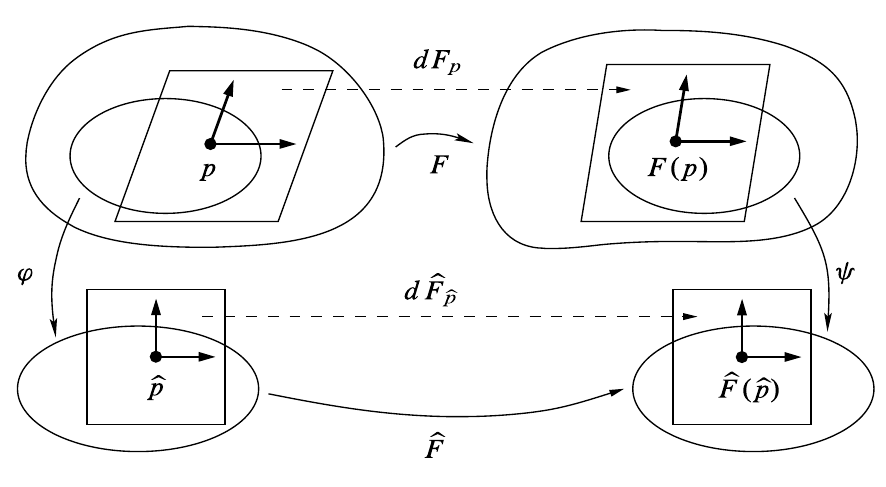
\includegraphics[scale = 0.5]{chapter03/c3f6.png}
\end{center}

\hl{\textbf{Note:}} In the differential geometry literature, the differential is sometimes called the \df{tangent map}, the \df{total derivative}, or simply the \df{derivative of F}. It can also sometimes be called the \df{(pointwise) pushforward}. Different authors denote it using symbols such as
\[F\p(p),\quad DF,\quad DF(p),\quad F_*,\quad TF, \quad T_pF.\]
However, we will stick to the notation $dF_p$.

\dfn Suppose $(U,\vphi)$ and $(V,\psi)$ are two smooth charts on $M$, and $p\in U\cap V$. Let us denote the coordinate functions of $\vphi$ by $(x^i)$ and those of $\psi$ by $(\td x^i)$. Then any tangent vector at $p$ can be represented with respect to either basis $\lp\ev{\pdd{x^i}}{p}\rp$ or $\lp\ev{\pdd{\td x^i}}{p}\rp$. Using our transition map and the definition of coordinate vectors, \hl{we can compute that}
\[\ev{\pdd{x^i}}{p} = \pd{\td x^j}{x^i}(\wh p)\ev{\pdd{\td x^j}}{p}.\]

\begin{ex}[\hlo{Polar Coordinates}]
The transition map between polar coordinates and standard coordinates in suitable open subsets of the plane is given by $(x,y) = (r\cos(\theta),r\sin(\theta)$. Let $p = (r,\theta) = (2, \pi/2)$, and let $v\in T_p\R^2$ be the tangent vector whose polar coordinate representation is
\[v = 3\ev{\pdd{r}}{p} = \ev{\pdd{\theta}}{p}.\]
Applying the rule in the above definition, we get that
\begin{align*}
    \ev{\pdd{r}}{p} &= \cos\lp\frac{\pi}{2}\rp\ev{\pdd{x}}{p} + \sin\lp\frac{\pi}{2}\rp\ev{\pdd{y}}{p} = \ev{\pdd{y}}{p},\\
    \ev{\pdd{\theta}}{p} &= 
    -2\sin\lp\frac{\pi}{2}\rp\ev{\pdd{x}}{p} + 2\cos\lp\frac{\pi}{2}\rp\ev{\pdd{y}}{p} = -2\ev{\pdd{x}}{p},
\end{align*}
and thus $v$ has the following coordinate representation in standard coordinates:
\[v = 3\ev{\pdd{y}}{p} + 2\ev{\pdd{x}}{p}.\]
\end{ex}


\subsection{The Tangent Bundle}\nl

\dfn Given a smooth manifold $M$ with or without boundary, we define the \df{tangent bundle of M}, denoted by $TM$, to be the disjoint union of the tangent spaces at all points of $M$:
\[TM = \bigsqcup_{p\in M} T_pM.\]

\nb We usually write an element of this disjoint union as an ordered pair $(p,v)$ with $p\in M$ and $v\in T_pM$, and the tangent bundle comes equipped with a natural projection map $\pi:TM\ra M:(p,v)\mapsto p$.

\setcounter{thm}{17}

\begin{prop}
For any smooth $n$-manifold $M$, the tangent bundle $TM$ has a natural topology and a smooth structure that make it into a $2n$-dimensional smooth manifold. With respect to this structure, the projection $\pi:TM\ra M$ is smooth.
\end{prop}

\begin{center}
    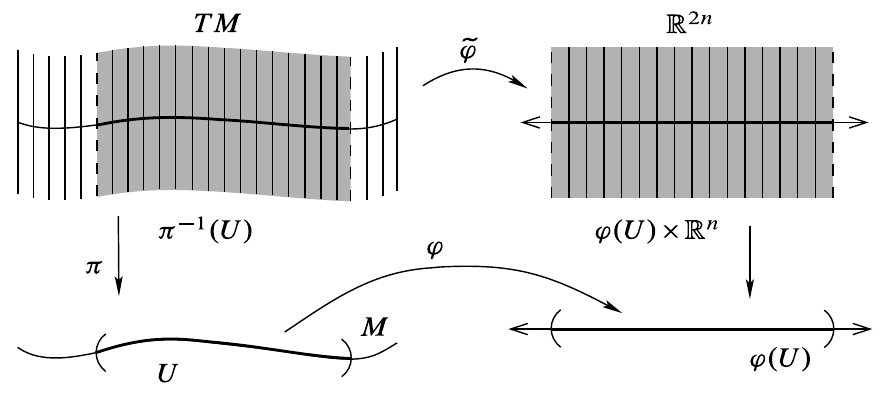
\includegraphics[scale = 0.5]{chapter03/c3f8.png}
\end{center}

\setcounter{thm}{19}

\begin{prop}
If $M$ is a smooth $n$-manifold with or without boundary, and $M$ can be covered by a single smooth chart, then $TM$ is diffoemorphic to $M\x \Rn$.
\end{prop}

\begin{prop}
If $F:M\ra N$ is a smooth map, then its global differential $dF:TM\ra TN$ is a smooth map.
\end{prop}

\begin{cor}[\hl{Properties of the Global Differential}]
Suppose $F:M\ra N$ and $G:N\ra P$ are smooth maps
\begin{enumerate}
    \item $d(G\circ F) = dG\circ dF$.
    \item $d(\Id_M) = \Id_{TM}$
    \item If $F$ is a diffeomorphism, then $dF:TM\ra TN$ is also a diffeomorphism, and $(dF)\inv = d(F\inv)$.
\end{enumerate}
\end{cor}

\dfn If $M$ is a manifold, a \df{curve in M} is a continuous map $\ga:J\ra M$, where $J\seq \R$ is an interval.

\dfn Given a smooth curve $\ga:J\ra M$, and $t_0\in J$, we define the \df{velocity of $\boldsymbol{\ga}$ at $\boldsymbol{t_0}$}, denoted by $\ga\p(t_0)$, to be the vector
\[\ga\p(t_0) = d\ga\lp\ev{\frac{d}{dt}}{t_0}\rp\in T_{\ga(t_0)}M,\]
where $\ev{\frac{d}{dt}}{t_0}$ is the standard coordinate basis vector in $T_{t_0}\R$.

\dfn Given a smooth chart $(U,(x^i))$ with $\ga(t_0)\in U$, we can write the coordinate representation of $\ga$ as $\ga(t) = (\ga^1(t),\ldots,\ga^n(t))$. Then the coordinate formula for the differential yields
\[\ga\p(t_0) = \frac{d\ga^i}{dt}(t_0)\ev{\pdd{x^i}}{\ga(t_0)}.\]

\begin{prop}
\hlb{Suppose $M$ is a smooth manifold with or without boundary and $p\in M$. Every $v\in T_pM$ is the velocity vector of some smooth curve in $M$.}
\end{prop}

\begin{prop}[The Velocity of a Composite Curve]
Let $F:M\ra N$ be a smooth map, and let $\ga:J\ra M$ be a smooth curve. For any $t_0\in J$, the velocity at $t = t_0$ of the composite curve $F\circ \ga:J\ra N$ is given by
\[(F\circ \ga)\p(t_0) = dF(\ga\p(t_0)).\]
\end{prop}

\begin{cor}[Computing the Differential Using a Velocity Vector]
Suppose $F:M\ra N$ is a smooth map, $p\in M$, and $v\in T_pM$. Then 
\[dF_p(v) = (F\circ \ga)\p(0)\]
for any smooth curve $\ga:J\ra M$ such that $0\in J, \ga(0) = p$, and $\ga\p(0) = v$.
\end{cor}






